\documentclass[aspectratio=169, 12pt, xcolor=table]{beamer}

% --- PAQUETES ---
\usepackage[utf8]{inputenc}
\usepackage[T1]{fontenc}
\usepackage[spanish, es-noshorthands, es-nodecimaldot]{babel}
\usepackage{tikz}
\usetikzlibrary{shapes.geometric, arrows.meta, positioning, fit, calc, decorations.pathreplacing, patterns}
\usepackage{pgfplots}
\pgfplotsset{compat=1.18}
\usepackage{helvet}
\usepackage{booktabs}
\usepackage{times}
\usepackage{amssymb}
\usepackage{appendixnumberbeamer}

% --- TEMA MINIMALISTA ---
\usetheme{default}
\usecolortheme{dove}
\useinnertheme{rectangles}
\setbeamertemplate{navigation symbols}{}
\setbeamersize{text margin left=0.6cm, text margin right=0.6cm}

\definecolor{SentricaBlue}{RGB}{0, 50, 100}
\definecolor{AlertRed}{RGB}{170, 30, 30}
\definecolor{Suave}{RGB}{220, 222, 230}
\setbeamercolor{title}{fg=SentricaBlue}
\setbeamercolor{frametitle}{fg=SentricaBlue}
\setbeamercolor{structure}{fg=SentricaBlue}
\setbeamercolor{block title}{fg=white, bg=SentricaBlue}
\setbeamercolor{block body}{bg=SentricaBlue!8}
\setbeamercolor{block title alerted}{fg=white, bg=AlertRed}
\setbeamercolor{block body alerted}{bg=AlertRed!8}
\setbeamerfont{frametitle}{size=\large, series=\bfseries}

% Barra de secciones arriba: la sección actual en azul.
\newcommand{\nav}[2]{\ifnum\value{section}=#1\textcolor{SentricaBlue}{\textbf{#2}}\else\textcolor{gray!55}{#2}\fi}
\setbeamertemplate{headline}{%
  \vskip5pt\hskip0.6cm{\scriptsize
    \nav{1}{Contenidos previos}\hspace{1.4em}\nav{2}{Estado del arte}\hspace{1.4em}%
    \nav{3}{Problema}\hspace{1.4em}\nav{4}{Objetivo}\hspace{1.4em}%
    \nav{5}{Reproducción}\hspace{1.4em}\nav{6}{Cierre}}}

% Número de diapositiva visible en todas: "n / total"
\setbeamertemplate{footline}{%
  \hfill\usebeamercolor[fg]{frametitle}\footnotesize\insertframenumber\,/\,\inserttotalframenumber\hspace{1.2em}\vspace{0.8em}}

% Etiqueta de fila en las líneas de tiempo
\newcommand{\fila}[2]{\node[anchor=east, font=\scriptsize, align=right] at (-0.15, #1+0.21) {#2};}

% Cita al pie de la diapositiva
\newcommand{\cita}[1]{\vfill{\tiny\color{gray}#1}}

% --- ESTILOS TIKZ ---
\tikzset{
  caja/.style={rectangle, draw=SentricaBlue, fill=gray!10, rounded corners, align=center, font=\scriptsize, minimum height=2.4em},
  cajaclave/.style={caja, fill=SentricaBlue!15, thick, font=\scriptsize\bfseries},
  flecha/.style={-Latex, thick, SentricaBlue},
  frame/.style={rectangle, draw=white, line width=0.3pt, minimum height=0.42cm, inner sep=0pt},
}

% --- METADATOS ---
\title{\textbf{Recuperación de video bajo pérdida\\sin lazo al codificador}}
\subtitle{Presentación de avance --- IPD438}
\author{Vicente Andrade Ercilla}
\institute{Universidad Técnica Federico Santa María}
\date{\today}

\begin{document}

% =====================================================================
\begin{frame}[plain]
    \titlepage
\end{frame}

% =====================================================================
\section{Contenidos previos}

\begin{frame}{Una pérdida dura hasta el próximo intra}
    \centering
    \vspace{0.2em}
    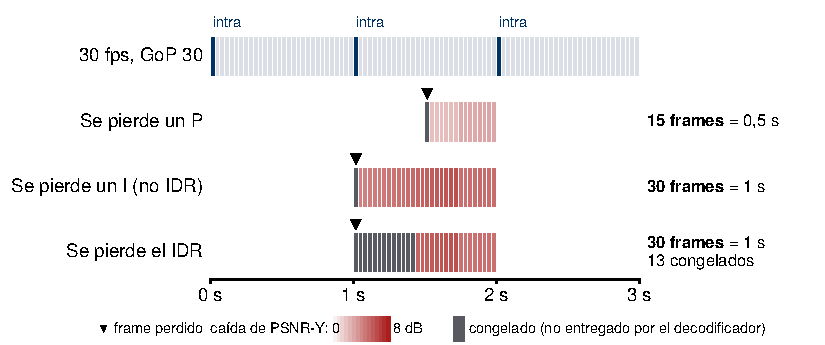
\includegraphics[width=\textwidth]{figuras/propagacion.pdf}

    \vspace{0.4em}
    {\scriptsize\color{gray} Medido: Big Buck Bunny 640$\times$360, x264 Baseline a 1 Mbps, una referencia, decodificador de FFmpeg.}
\end{frame}

% ---------------------------------------------------------------------
\begin{frame}{El IDR es el frame más grande, y el más expuesto}
    \centering
    \begin{tikzpicture}[x=1cm, y=1cm]
        \def\pq{0.125}   % ancho de un paquete de 1200 B
        % --- Flujo Annex B ---
        \node[anchor=east, font=\scriptsize\bfseries, text=SentricaBlue] at (1.3, 1.6) {H.264 Annex B};
        \node[frame, fill=gray!35, minimum width=0.5cm, font=\tiny] at (1.75, 1.6) {SPS};
        \node[frame, fill=gray!35, minimum width=0.5cm, font=\tiny] at (2.27, 1.6) {PPS};
        \node[frame, fill=SentricaBlue, minimum width=47*\pq cm, anchor=west, text=white, font=\scriptsize] (idr) at (2.55, 1.6) {IDR \;·\; 55 kB};
        \foreach \k in {0,...,7}{
            \node[frame, fill=Suave, minimum width=2*\pq cm, anchor=west] (p\k) at ({2.6 + 47*\pq + \k*(2*\pq+0.07)}, 1.6) {};
        }
        \node[font=\tiny, anchor=west] at ({2.65 + 47*\pq + 8*(2*\pq+0.07)}, 1.6) {\dots};
        \node[font=\tiny, text=gray, below=1pt of p3.south east] {P $\approx$ 2 kB};
        % SEI
        \node[frame, fill=AlertRed!70, minimum width=0.12cm, anchor=west] (sei) at ({2.6 + 47*\pq + 5*(2*\pq+0.07) - 0.1}, 1.6) {};
        \draw[AlertRed, thin] (sei.north) -- ++(0, 0.4) node[above, font=\scriptsize, align=center, text=AlertRed] {SEI: datos que el\\decodificador puede ignorar};

        % --- Paquetes RTP ---
        \node[anchor=east, font=\scriptsize\bfseries, text=SentricaBlue] at (1.3, 0.5) {RTP (FU-A)};
        \foreach \i in {0,...,46}{
            \fill[SentricaBlue!55] ({2.55 + \i*\pq + 0.012}, 0.32) rectangle ++({\pq - 0.024}, 0.36);
        }
        \fill[AlertRed] ({2.55 + 20*\pq + 0.012}, 0.32) rectangle ++({\pq - 0.024}, 0.36);
        \node[text=AlertRed, font=\bfseries\small] at ({2.55 + 20.5*\pq}, 0.95) {$\times$};
        \foreach \k in {0,...,7}{
            \foreach \j in {0,1}{
                \fill[gray!45] ({2.6 + 47*\pq + \k*(2*\pq+0.07) + \j*\pq + 0.012}, 0.32) rectangle ++({\pq - 0.024}, 0.36);
            }
        }
        \draw[decorate, decoration={brace, mirror, amplitude=3pt}, SentricaBlue]
            (2.55, 0.22) -- ({2.55 + 47*\pq}, 0.22) node[midway, below=4pt, font=\scriptsize] {47 paquetes: perder uno rompe el IDR};
        \node[font=\scriptsize, anchor=north] at ({2.6 + 47*\pq + 1.4}, 0.22) {2 paquetes por P};
    \end{tikzpicture}

    \vspace{0.1em}
    {\scriptsize\color{gray} Tipo de NAL: 1 = P,\enspace 5 = IDR,\enspace 6 = SEI,\enspace 7 = SPS,\enspace 8 = PPS. \enspace Paquetes de 1200 B; mismo clip.}

    \vspace{0.7em}
    \begin{tikzpicture}
        \node[caja, minimum width=4.2cm, minimum height=3.2em] (a) {{\Large\bfseries 38 \%}\\ P(dañar el IDR) con 1 \% de pérdida};
        \node[caja, minimum width=4.2cm, minimum height=3.2em, right=0.4cm of a] (b) {{\Large\bfseries 2 \%}\\ P(dañar un P)};
        \node[caja, minimum width=4.2cm, minimum height=3.2em, right=0.4cm of b] (c) {{\Large\bfseries 1 de 3}\\ paquetes es de un IDR};
    \end{tikzpicture}
\end{frame}

% =====================================================================
\section{Estado del arte}

\begin{frame}{Hoy, recuperarse exige lazo al codificador o pagar siempre}
    \centering
    {\scriptsize\color{gray} Si NACK o FEC no alcanzan (plazo de latencia, ráfagas), el decodificador queda desincronizado.}

    \vspace{0.5em}
    \begin{tikzpicture}[x=1cm, y=1cm]
        \def\W{5.6} \def\H{1.85}
        % Encabezados
        \node[font=\footnotesize\bfseries, text=SentricaBlue] at (0.5*\W, 2*\H + 0.3) {Con lazo al codificador};
        \node[font=\footnotesize\bfseries, text=SentricaBlue] at (1.5*\W + 0.15, 2*\H + 0.3) {Sin lazo al codificador};
        \node[font=\footnotesize\bfseries, text=SentricaBlue, anchor=east, align=right] at (-0.2, 1.5*\H + 0.1) {Cuesta con\\la red sana};
        \node[font=\footnotesize\bfseries, text=SentricaBlue, anchor=east, align=right] at (-0.2, 0.5*\H) {No cuesta con\\la red sana};
        % Celdas
        \draw[SentricaBlue, fill=gray!8, rounded corners] (0, \H + 0.15) rectangle (\W, 2*\H + 0.05);
        \draw[SentricaBlue, fill=gray!8, rounded corners] (\W + 0.15, \H + 0.15) rectangle (2*\W + 0.15, 2*\H + 0.05);
        \draw[SentricaBlue, fill=gray!8, rounded corners] (0, 0) rectangle (\W, \H);
        \draw[AlertRed, very thick, dashed, fill=AlertRed!6, rounded corners] (\W + 0.15, 0) rectangle (2*\W + 0.15, \H);
        % Contenido
        \node[align=center, font=\scriptsize] at (0.5*\W, 1.5*\H + 0.1) {\textbf{GoP adaptativo} --- FrameTrace [1]\\[0.15em]el receptor reporta pérdida y el\\codificador acorta el GoP para todos};
        \node[align=center, font=\scriptsize] at (1.5*\W + 0.15, 1.5*\H + 0.1) {\textbf{GoP corto}\\\textbf{Intra refresh} + Recovery Point SEI\\\textbf{Redundant pictures} (H.264)\\[0.15em]se refresca siempre, haya o no pérdida};
        \node[align=center, font=\scriptsize] at (0.5*\W, 0.5*\H) {\textbf{PLI / FIR}: el receptor pide un IDR\\[0.15em]\textbf{LTR + RPSI}: predecir desde una\\referencia que el receptor confirmó};
        \node[font=\Huge\bfseries, text=AlertRed] at (1.5*\W + 0.15, 0.5*\H) {?};
    \end{tikzpicture}

    \vspace{0.4em}
    {\scriptsize\color{gray} En 1-a-muchos (CDN), el IDR que pide un receptor lo reciben y lo pagan todos.}
\end{frame}

% ---------------------------------------------------------------------
\begin{frame}{FrameTrace [1]: el GoP corto salva la calidad bajo pérdida}
    \begin{columns}[T]
        \begin{column}{0.48\textwidth}
            \centering
            {\footnotesize\textbf{GoP corto bajo pérdida}}\\[-0.2em]
            {\tiny\color{gray} Big Buck Bunny 720p, 1 \% de pérdida, 500 ms de retardo}

            \begin{tikzpicture}
                \begin{axis}[
                    width=6.2cm, height=4.6cm, ybar, bar width=1.1cm,
                    ymin=0, ymax=100, ylabel={VMAF}, ylabel style={font=\scriptsize},
                    symbolic x coords={GoP 0{,}5 s, GoP 2 s}, xtick=data,
                    enlarge x limits=0.5, axis lines*=left,
                    tick label style={font=\scriptsize},
                    nodes near coords, nodes near coords style={font=\footnotesize\bfseries},
                    /pgf/number format/use comma,
                ]
                    \addplot[fill=SentricaBlue, draw=none] coordinates {(GoP 0{,}5 s, 72.6) (GoP 2 s, 55.7)};
                \end{axis}
            \end{tikzpicture}
        \end{column}
        \begin{column}{0.48\textwidth}
            \centering
            {\footnotesize\textbf{Su controlador acorta el GoP}}\\[-0.2em]
            {\tiny\color{gray} con realimentación del cliente (FDR) al codificador}

            \begin{tikzpicture}
                \begin{axis}[
                    width=6.2cm, height=4.6cm, ybar, bar width=0.8cm,
                    ymin=0, ymax=2.5, ylabel={GoP medio (s)}, ylabel style={font=\scriptsize},
                    symbolic x coords={0 \%, 10 \%, 20 \%}, xtick=data,
                    xlabel={pérdida}, xlabel style={font=\scriptsize},
                    enlarge x limits=0.3, axis lines*=left,
                    tick label style={font=\scriptsize},
                    nodes near coords, nodes near coords style={font=\footnotesize\bfseries},
                    /pgf/number format/use comma, /pgf/number format/precision=2,
                ]
                    \addplot[fill=AlertRed!75, draw=none] coordinates {(0 \%, 2.02) (10 \%, 1.56) (20 \%, 0.88)};
                \end{axis}
            \end{tikzpicture}
        \end{column}
    \end{columns}

    \vspace{0.2em}
    \centering
    {\scriptsize Métrica que tomo de [1]: \textbf{FRR} = frames mostrados / frames enviados (ocultar congelando no cuenta como ganar).}

    \cita{[1] B. Denizer, L. Winkel, O. Landsiedel. \emph{FrameTrace: Frame-Level Telemetry for Media over QUIC}. EMS '25, ACM SIGCOMM 2025, pp. 31--36.}
\end{frame}

% ---------------------------------------------------------------------
\begin{frame}{AGiLE [2]: GoP largo, puntos de entrada cada 2 s}
    \centering
    \begin{tikzpicture}[x=1.15cm, y=1cm]
        % Flujo: GoP de 10 s con I-headers cada 2 s
        \fill[Suave] (0, 0) rectangle (10, 0.42);
        \fill[SentricaBlue] (0, 0) rectangle (0.12, 0.42);
        \fill[SentricaBlue] (10, 0) rectangle (10.12, 0.42);
        \foreach \t in {2,4,6,8}{
            \draw[AlertRed] (\t, 0.42) -- (\t, 0.7);
            \node[rectangle, draw=AlertRed, fill=AlertRed!15, font=\tiny\bfseries, minimum size=0.36cm, inner sep=0pt] (ih\t) at (\t, 0.9) {I};
        }
        \node[font=\scriptsize, text=AlertRed, anchor=south, align=center] at (5, 1.12) {I-header: la misma imagen codificada también como I, dentro de un SEI};
        \foreach \s in {0,2,...,10}{ \node[font=\tiny, text=gray, below] at (\s, 0) {\s\,s}; }
        \draw[decorate, decoration={brace, mirror, amplitude=3pt}, AlertRed] (2, -0.35) -- (4, -0.35) node[midway, below=3pt, font=\scriptsize] {pseudo-GOP: 2 s};
        \draw[decorate, decoration={brace, mirror, amplitude=4pt}, SentricaBlue] (0, -0.95) -- (10.12, -0.95) node[midway, below=4pt, font=\scriptsize] {GoP de codificación: 10 s};

        % Edge y espectadores
        \node[cajaclave, minimum width=2.2cm] (edge) at (2.2, -2.3) {Edge\\guarda el I-header};
        \node[caja, minimum width=4.6cm, anchor=west, minimum height=1.9em] (nuevo) at (4.6, -1.9) {Espectador \textbf{nuevo}: I-header + P siguientes \textcolor{SentricaBlue}{$\checkmark$}};
        \node[caja, minimum width=4.6cm, anchor=west, minimum height=1.9em, draw=AlertRed] (con) at (4.6, -2.7) {Espectador \textbf{conectado}: el I-header \textcolor{AlertRed}{se descarta}};
        \draw[flecha] (edge.east) -- (nuevo.west);
        \draw[-Latex, thick, AlertRed, dashed] (edge.east) -- (con.west);
    \end{tikzpicture}

    \vspace{0.2em}
    \begin{tikzpicture}
        \node[caja, minimum width=4.2cm, minimum height=3em] (a) {{\large\bfseries $-$3,5 \%} BD-bitrate\\vs GoP fijo de 2 s};
        \node[caja, minimum width=4.2cm, minimum height=3em, right=0.4cm of a] (b) {{\large\bfseries +2,8 \%} de datos\\en ingest (I-headers)};
        \node[caja, minimum width=4.2cm, minimum height=3em, right=0.4cm of b] (c) {{\large\bfseries 1,1 VMAF} de deriva\\hasta el próximo I real};
    \end{tikzpicture}

    \cita{[2] C. Chen, W. Yin, Z. Huang, S. Shi. \emph{AGiLE: Enhancing Adaptive GOP in Live Video Streaming}. MMSys '24, pp. 34--44.}
\end{frame}

% =====================================================================
\section{Problema}

\begin{frame}{Anomalía: el I-header ya está en el edge, y se descarta}
    \centering
    \begin{tikzpicture}[x=1.05cm, y=1cm]
        % Estructura
        \fila{2.4}{Flujo (AGiLE)}
        \fill[Suave] (0, 2.4) rectangle (10, 2.82);
        \fill[SentricaBlue] (0, 2.4) rectangle (0.12, 2.82);
        \fill[SentricaBlue] (10, 2.4) rectangle (10.12, 2.82);
        \foreach \t in {2,4,6,8}{
            \node[rectangle, draw=AlertRed, fill=AlertRed!15, font=\tiny\bfseries, minimum size=0.32cm, inner sep=0pt] at (\t, 3.05) {I};
        }
        \foreach \s in {0,2,...,10}{ \node[font=\tiny, text=gray] at (\s, 2.25) {\s\,s}; }

        % Hoy: espectador con pérdida
        \fila{1.25}{Con pérdida, hoy}
        \fill[Suave] (0, 1.25) rectangle (2.5, 1.67);
        \fill[AlertRed!80] (2.5, 1.25) rectangle (10, 1.67);
        \fill[SentricaBlue] (10, 1.25) rectangle (10.12, 1.67);
        \node[text=white, font=\scriptsize\bfseries] at (6.25, 1.46) {7,5 s dañado: hasta el próximo I real};
        \node[font=\scriptsize] at (2.5, 1.85) {$\blacktriangledown$};
        \node[rectangle, draw=AlertRed, fill=white, font=\tiny\bfseries, minimum size=0.32cm, inner sep=0pt] (desc) at (4, 1.9) {I};
        \draw[AlertRed, thick] (desc.south west) -- (desc.north east) (desc.north west) -- (desc.south east);
        \node[font=\tiny, text=AlertRed, anchor=west] at (4.2, 1.95) {descartado};

        % Propuesta
        \fila{0.1}{Con pérdida,\\si se le entrega}
        \fill[Suave] (0, 0.1) rectangle (2.5, 0.52);
        \fill[AlertRed!80] (2.5, 0.1) rectangle (4, 0.52);
        \fill[pattern=north east lines, pattern color=AlertRed!45] (4, 0.1) rectangle (10, 0.52);
        \fill[SentricaBlue] (10, 0.1) rectangle (10.12, 0.52);
        \node[font=\scriptsize] at (2.5, 0.7) {$\blacktriangledown$};
        \node[rectangle, draw=AlertRed, fill=AlertRed!15, font=\tiny\bfseries, minimum size=0.32cm, inner sep=0pt] at (4, 0.75) {I};
        \node[font=\scriptsize\bfseries, text=AlertRed, anchor=north] at (3.25, 0.05) {1,5 s};
        \node[font=\scriptsize, text=gray, anchor=north] at (7, 0.05) {deriva leve ($\approx$ 1 VMAF)};
    \end{tikzpicture}

    \vspace{0.6em}
    \begin{alertblock}{Idea fuerte}
        \centering
        El mecanismo para recuperarse de la pérdida ya está en la red,
        ya está pagado, y hoy se descarta.
    \end{alertblock}

    {\tiny\color{gray} Esquema con los parámetros de AGiLE (GoP 10 s, pseudo-GOP 2 s) y transporte que descarta lo que llega tarde (RTP, SRT, MoQ).}
\end{frame}

% =====================================================================
\section{Objetivo}

\begin{frame}{Objetivo: medir cuánto daño ahorra entregar el I-header}
    \centering
    {\small Al término del semestre: demostrar en una plataforma real que entregar el I-header\\a los receptores con pérdida acorta el daño, \textbf{sin lazo al codificador}.}

    \vspace{0.8em}
    \begin{tikzpicture}[node distance=0.45cm]
        \node[caja, minimum width=2.6cm] (tx) {STM32\\H.264 + I-header};
        \node[cajaclave, minimum width=2.6cm, right=of tx] (ed) {Edge\\lee SEI y decide};
        \node[caja, minimum width=2.6cm, right=of ed, draw=AlertRed] (ch) {Última milla\\pérdida (tc-netem)};
        \node[caja, minimum width=2.6cm, right=of ch] (rx) {Receptor\\métricas por frame};
        \draw[flecha] (tx) -- (ed);
        \draw[flecha] (ed) -- (ch);
        \draw[flecha] (ch) -- (rx);
    \end{tikzpicture}

    \vspace{0.8em}
    \footnotesize
    \renewcommand{\arraystretch}{1.15}
    \newcommand{\q}{\textcolor{gray!60}{?}}
    \begin{tabular}{l c c c c}
        \toprule
        \textbf{Mismo perfil de pérdida} & \textbf{Duración} & \textbf{Severidad} & \textbf{Congelamiento} & \textbf{Costo con} \\
        & {\scriptsize frames} & {\scriptsize VMAF} & {\scriptsize FRR} & \textbf{red sana} \\
        \midrule
        GoP largo, sin protección & \q & \q & \q & ninguno \\
        GoP corto / intra refresh & \q & \q & \q & siempre \\
        PLI (lazo al codificador) & \q & \q & \q & ninguno \\
        \rowcolor{SentricaBlue!12}
        \textbf{Propuesta: I-header al dañado} & \q & \q & \q & \textbf{ninguno} \\
        \bottomrule
    \end{tabular}
\end{frame}

% =====================================================================
\section{Reproducción}

\begin{frame}{Para la final: reproducir la Fig.~12 de AGiLE en H.264}
    \begin{columns}[c]
        \begin{column}{0.47\textwidth}
            \footnotesize
            \begin{tikzpicture}[node distance=0.16cm]
                \tikzset{paso/.style={caja, minimum width=6.2cm, minimum height=1.9em, align=left, text width=5.9cm}}
                \node[paso, fill=SentricaBlue!12] (a) {\textcolor{SentricaBlue}{$\checkmark$} Codificar con x264: Baseline, 1 referencia};
                \node[paso, fill=SentricaBlue!12, below=of a] (b) {\textcolor{SentricaBlue}{$\checkmark$} Forzar un I no-IDR en la frontera};
                \node[paso, fill=SentricaBlue!12, below=of b] (c) {\textcolor{SentricaBlue}{$\checkmark$} Quitar frames del Annex B y medir};
                \node[paso, below=of c] (d) {\textcolor{gray}{$\circ$} Reemplazar el P por el I-header};
                \node[paso, below=of d] (e) {\textcolor{gray}{$\circ$} VMAF por I-header de entrada};
            \end{tikzpicture}

            \vspace{0.3em}
            {\scriptsize\color{gray} $\checkmark$ ya funciona (figura de la diapositiva 2)}
        \end{column}
        \begin{column}{0.5\textwidth}
            \centering
            \begin{tikzpicture}
                \begin{axis}[
                    width=7cm, height=5.2cm,
                    xmin=0.5, xmax=4.5, ymin=0, ymax=3,
                    xtick={1,2,3,4}, xticklabels={1.\textsuperscript{o}, 2.\textsuperscript{o}, 3.\textsuperscript{o}, 4.\textsuperscript{o}},
                    xlabel={I-header por el que se entra}, ylabel={caída de VMAF},
                    label style={font=\scriptsize}, tick label style={font=\scriptsize},
                    axis lines*=left, /pgf/number format/use comma,
                ]
                    \addplot[only marks, mark=*, mark size=2.5pt, SentricaBlue] coordinates {(1, 1.1)};
                    \node[font=\scriptsize, text=SentricaBlue, anchor=south west] at (axis cs:1.05, 1.15) {AGiLE, H.265: 1,1};
                    \draw[gray, dashed] (axis cs:0.5, 2.64) -- (axis cs:4.5, 2.64) node[pos=0.98, above, font=\tiny, anchor=south east] {peor caso en AGiLE: 2,64};
                    \addplot[only marks, mark=none, nodes near coords={?},
                        nodes near coords style={font=\small\bfseries, text=AlertRed, anchor=center}]
                        coordinates {(1, 0.45) (2, 0.45) (3, 0.45) (4, 0.45)};
                    \node[font=\tiny, text=AlertRed] at (axis cs:2.5, 0.8) {H.264 (este trabajo): por medir};
                \end{axis}
            \end{tikzpicture}

            {\scriptsize En AGiLE, la caída disminuye del 1.\textsuperscript{o} al 4.\textsuperscript{o} I-header.}
        \end{column}
    \end{columns}
\end{frame}

% =====================================================================
\section{Cierre}

\begin{frame}{Qué recordar}
    \centering
    \vspace{0.6em}
    {\large\color{SentricaBlue}\textbf{Recuperarse de la pérdida sin pedirle nada al codificador,\\usando un punto de recuperación que ya está en la red.}}

    \vspace{1.6em}
    \begin{tikzpicture}
        \node[caja, minimum width=4.3cm, minimum height=4.6em, text width=4cm] (a) {{\Large\bfseries 1 s}\\ dañado por perder un IDR\\(30 fps, GoP 30; 13 frames congelados)};
        \node[caja, minimum width=4.3cm, minimum height=4.6em, text width=4cm, right=0.35cm of a] (b) {{\Large\bfseries lazo o costo}\\ lo que hoy exige\\recuperarse};
        \node[cajaclave, minimum width=4.3cm, minimum height=4.6em, text width=4cm, right=0.35cm of b] (c) {{\Large 10 s $\rightarrow$ 2 s}\\{\normalfont daño máximo con el GoP de AGiLE,\\sin y con I-header}};
    \end{tikzpicture}
\end{frame}

% =====================================================================
\appendix
\setbeamertemplate{headline}{\vskip5pt\hskip0.6cm{\scriptsize\textcolor{gray!55}{Respaldo}}}

\begin{frame}{Referencias}
    \footnotesize
    \setlength{\itemsep}{0pt}
    \textbf{Estado del arte}
    \begin{itemize}
        \item[{[1]}] B. Denizer, L. Winkel, O. Landsiedel. \emph{FrameTrace: Frame-Level Telemetry for Media over QUIC}. EMS '25, ACM SIGCOMM 2025, pp. 31--36. doi:10.1145/3746441.3748231
        \item[{[2]}] C. Chen, W. Yin, Z. Huang, S. Shi. \emph{AGiLE: Enhancing Adaptive GOP in Live Video Streaming}. MMSys '24, pp. 34--44. doi:10.1145/3625468.3647609
    \end{itemize}

    \textbf{Base teórica}
    \begin{itemize}
        \item[{[3]}] T. Wiegand, G. Sullivan, G. Bjøntegaard, A. Luthra. \emph{Overview of the H.264/AVC video coding standard}. IEEE TCSVT, 2003.
        \item[{[4]}] Y. Wang, Q.-F. Zhu. \emph{Error control and concealment for video communication: a review}. Proc. IEEE, 1998.
        \item[{[5]}] ITU-T Rec. H.264. \emph{Advanced video coding for generic audiovisual services} (Anexos B y D).
        \item[{[6]}] RFC 6184. \emph{RTP Payload Format for H.264 Video}, 2011.
        \item[{[7]}] RFC 8834. \emph{Media Transport and Use of RTP in WebRTC}, 2021.
    \end{itemize}
\end{frame}

% ---------------------------------------------------------------------
\begin{frame}{Por qué perder el IDR es peor que perder un I}
    \centering
    \begin{tikzpicture}[x=0.42cm, y=1cm]
        \foreach \i/\fn in {27/11, 28/12, 29/13}{
            \node[frame, fill=Suave, minimum width=0.4cm, font=\tiny] at (\i, 1) {\fn};
        }
        \node[frame, fill=AlertRed!25, minimum width=0.4cm, font=\tiny] at (30, 1) {0};
        \node[text=AlertRed, font=\bfseries] at (30, 1.55) {$\times$};
        \foreach \i/\fn in {31/1, 32/2, 33/3, 34/4}{
            \node[frame, fill=Suave, minimum width=0.4cm, font=\tiny] at (\i, 1) {\fn};
        }
        \node[font=\tiny] at (35.3, 1) {\dots};
        \node[anchor=east, font=\scriptsize] at (26.3, 1) {frame\_num};
        \node[font=\tiny, text=AlertRed, below] at (30, 0.7) {IDR: reinicia a 0};
    \end{tikzpicture}

    \vspace{0.6em}
    \small
    \begin{itemize}
        \item El IDR vacía el DPB y reinicia \texttt{frame\_num} y POC. Un I no-IDR no.
        \item Si se pierde el IDR, el decodificador ve \texttt{frame\_num} 13 $\rightarrow$ 1, rellena el hueco y no detecta el reinicio: calcula POC menores que los ya mostrados.
        \item FFmpeg los descarta por desordenados: \textbf{12 frames congelados}, después artefactos hasta el próximo IDR.
        \item Si se pierde un I no-IDR, solo hay un hueco de 1 frame: oculta y sigue (artefactos, sin congelar).
    \end{itemize}
    {\scriptsize\color{gray} Comportamiento medido con FFmpeg 6.1; otros decodificadores pueden reaccionar distinto.}
\end{frame}

% ---------------------------------------------------------------------
\begin{frame}{¿Cómo sabe el edge a quién entregarlo?}
    \small
    \begin{columns}[T]
        \begin{column}{0.32\textwidth}
            \begin{block}{(a) El receptor avisa}
                Lazo corto al edge, no al codificador.\\[0.3em]
                {\scriptsize Compite con NACK y PLI; debilita el título.}
            \end{block}
        \end{column}
        \begin{column}{0.32\textwidth}
            \begin{block}{(b) El edge infiere}
                Retransmisiones, ACK faltantes, congestión de la última milla.\\[0.3em]
                {\scriptsize Versión fuerte; depende del protocolo.}
            \end{block}
        \end{column}
        \begin{column}{0.32\textwidth}
            \begin{alertblock}{(c) Siempre a todos}
                Cero lazo, pero se pierde el ahorro.\\[0.3em]
                {\scriptsize Equivale a GoP corto: no sirve.}
            \end{alertblock}
        \end{column}
    \end{columns}

    \vspace{1em}
    \centering
    Es la pregunta central del trabajo: la plataforma permite comparar (a) y (b).
\end{frame}

% ---------------------------------------------------------------------
\begin{frame}{Costos: qué se pierde}
    \footnotesize
    \renewcommand{\arraystretch}{1.25}
    \begin{tabular}{>{\bfseries}p{3.2cm} p{10.6cm}}
        \toprule
        Exactitud & Deriva hasta el próximo I real (AGiLE: $\approx$1,1 VMAF; peor caso 2,64). \\
        Ráfaga & Un intra pesa $\sim$20 P (clip medido) y se envía justo cuando el enlace está perdiendo. \\
        Doble codificación & Dos contextos de codificador en el STM32 (cómputo, memoria, energía). \\
        Ingest & +2,8 \% de datos (AGiLE, H.265); en H.264 hay que medirlo. \\
        Estado en el edge & ``Sin lazo al codificador'' $\neq$ ``sin estado''. \\
        Granularidad & Solo se recupera en fronteras de pseudo-GOP. \\
        Contenido & El GoP largo pierde eficiencia con mucho movimiento. \\
        Compatibilidad & Decodificadores que no arrancan desde un I no-IDR sin Recovery Point SEI. \\
        \bottomrule
    \end{tabular}
\end{frame}

\end{document}
